\section{Theoretic Foundations}
\label{sec:Theorie}

\subsection{The LHCb detector}

The LHCb experiment is one of the four larg experiments located at the Large Hadrom Collider (LHC) at CERN. 
This analysis is concerned with data from proton collisions from run 2 (2015-2018) of the experiment where proton bunches were collided at 
a center of mass energy of $13 \, \si{\tera\eV}$ with a frequency of $40 \cdot 10^6 \, \si{\hertz}$. The LHCb experiment studies mainly hadrons 
containing a charm or a bottom quark. It allows precision measurments of flavor physics processes. 
The composition of the LHCb detector is shown in figure \ref{f1}. 
\begin{figure}[!htb]
    \centering
    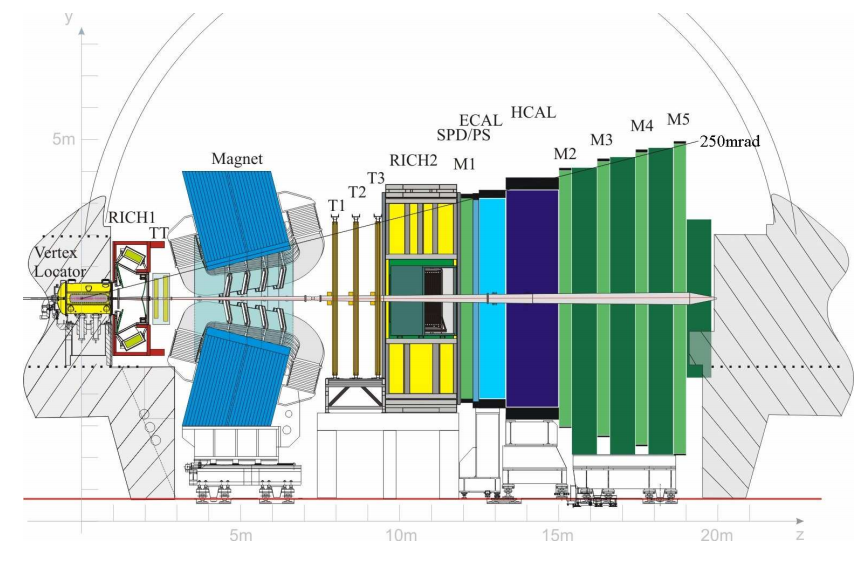
\includegraphics[width=0.8\textwidth]{graphics/lhcb.png}
    \caption{Components of the LHCb detector. \cite{sample_cpv}}
    \label{f1}
  \end{figure}










\subsection{The $B_s^0$ decay}
The stdied decay in this aalysis is $B_s^0 \rightarrow \psi(2S) K_s^0$. Since this decay is flavor chancing it must be a weak decay. 
A leading order feynman diagram is shown in figure \ref{f2}. Since the decay products are not measured directly the secondary decays have to be discussed. \\
The quark content of $\psi(2S)$ is $c \overline{c}$ and it decays dominantly via the strong interaction. To reduce errors due to misidentification of 
particles the electromagnetic decay $\psi(2S) \rightarrow \mu^+ \mu^-$ with a branching fraction of $\mathcal{B}(\psi(2S) \rightarrow \mu^+ \mu^-) 
(8.0 \pm 0.6) \cdot 10^{-3}$ \cite{pdg} will be used in the analysis. To exclude other particles containing $c\overline{c}$ 
the invariant mass of the muons is restricted to $m(\mu^+ \mu^- ) \approx m(\psi(2S))$ .\\ 
The $K_s^0$ has as quark content a superposition of $d \overline{s}$ and $\overline{d}s$. The dominant decay mode, which will be used in the analysis, 
is $K_s^0 \rightarrow \pi^+ \pi^-$ with a branching fraction of $\mathcal{B}(K_s^0 \rightarrow \pi^+ \pi^-) = (69.20 \pm 0.05) \, \%$ \cite{pdg}. \\
The data contains a significant number of background events from combinatorial background and the decay $B^0 \rightarrow \psi(2S) K_s^0$. 
The decay $B^0 \rightarrow \psi(2S) K_s^0$ is kinematically similar to the studied decay and passes all the selection criteria discussed so far. 
The invariant mass of the $B^0$ events shows a sharp peak that is smeared out due to the detector resolution. 
Combinatorial background results from wrongly combined events that do not originate from the decay of the $B^0$. The invariant mass of the 
combinatorial background is distributet randomly. 
To separate the signal from the decay $B_s^0 \rightarrow \psi(2S) K_s^0$ from the various backgrounds a Boosted Decion Tree (BDT) is implemented. 

  \begin{figure}[!htb]
    \centering
    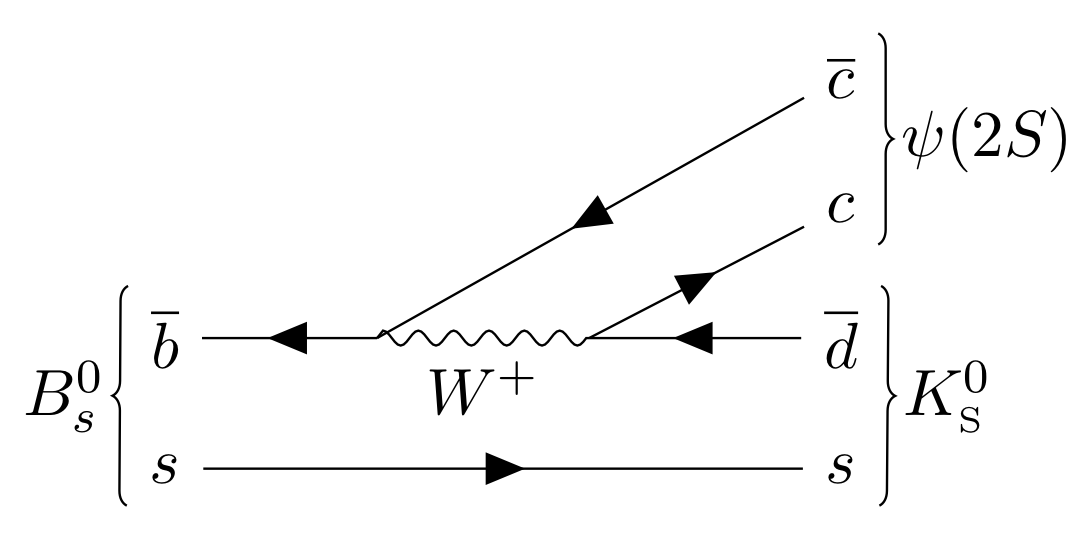
\includegraphics[width=0.4\textwidth]{graphics/image.png}
    \caption{A leading order feynman diagram for the decay $B_s^0 \rightarrow \psi(2S) K_s^0$. \cite{sample}}
    \label{fig:lhcb}
  \end{figure}